\documentclass{beamer}
\usetheme{Warsaw}

\usepackage[utf8]{inputenc}
\usepackage{fancybox}
\usepackage{multimedia} 
\usepackage{subfig}
\usepackage{amsmath}
\usepackage{hyperref}
\usepackage[all]{xy}
\begin{document}


\title[Stochastik] % (optional, only for long titles)
{Stochastik für Informatiker
\\
\includegraphics[scale=0.5]{img/craps}
}
\subtitle{}
\author[Dr. Johannes Riesterer] % (optional, for multiple authors)
{Dr.  rer. nat. Johannes Riesterer}

\date[KPT 2004] % (optional)
{}

\subject{Stochastik}

\frame{\titlepage}

\begin{frame}
    \frametitle{Übungsaufgaben}
\framesubtitle{}
\begin{block}{Aufgabe}
Beim Lottospiel werden ohne zurücklegen $6$ Zahlen aus $49$ gezogen. Berechnen Sie die folgenden Wahrscheinlichkeiten:
\begin{enumerate}
\item Alle $6$ Gewinnzahlen richtig zu tippen.
\item Genau $5$ richtige Gewinnzahlen zu tippen.
\item Mindestens $3$ richtige Gewinnzahlen zu tippen.
\item Alle $6$ Gewinnzahlen sind gerade.
\end{enumerate}
\end{block}
 \end{frame}

\begin{frame}
    \frametitle{Lösung}
\framesubtitle{}
 Der Grundraum beim Lottospiel ist eine Kombination ohne Beachtung der Reihenfolge
$\Omega = \{ (z_1, \dots,  z_6);  z_i \in \{1, \cdots, 49 \} , z_1 < z_2 < \cdots < z_6 \}$ und damit ist $| \Omega| = \begin{pmatrix} 
    49 \\ 6 \end{pmatrix} = 13983816$.
Die Anzahl $A_i$ an Kombinationen $i$  Zahlen aus $6$ richtigen zu tippen ist $ \begin{pmatrix} 
    6 \\ i \end{pmatrix} \cdot \begin{pmatrix} 
    43   \\ 6 -i \end{pmatrix}$ ($i$ Zahlen von $6$ richtig Tippen mal $6-i$ Zahlen von den falschen $49-6$ Zahlen zu tippen)

1) $ | A_6 |  = 1 \Rightarrow P(A_6) = \frac{1}{|\Omega|}  \approx 7,14 \cdot 10^{-8}$
\\ 2) $ | A_5 |  =  \begin{pmatrix} 
    6 \\ 5 \end{pmatrix} \cdot \begin{pmatrix} 
    43   \\ 1 \end{pmatrix} = 258 \Rightarrow P(A_5) = \frac{258}{|\Omega|}   \approx 1,845 \cdot 10^{-5}$
\\ 3) $B = \{ \text{mindestens 3 richtig}\} = A_6 \cup A_5 \cup A_4 \cup A_3$.   $P(B) = P (A_6 \cup A_5 \cup A_4 \cup A_3)= P(A_6) + P(A_5) + P(A_4) + P(A_3)$, da $A_i$ paarweise disjunkt.
 $ | A_4 |  =  \begin{pmatrix} 
    6 \\ 4 \end{pmatrix} \cdot \begin{pmatrix} 
    43   \\ 2 \end{pmatrix} = 13545 \Rightarrow P(A_4) = \frac{13545}{|\Omega|}   \approx 9,69 \cdot 10^{-4}$

 \end{frame}

\begin{frame}
    \frametitle{Lösung}
\framesubtitle{}
 $ | A_3 |  =  \begin{pmatrix} 
    6 \\ 3 \end{pmatrix} \cdot \begin{pmatrix} 
    43   \\ 3 \end{pmatrix} = 246820 \Rightarrow P(A_4) = \frac{246820}{|\Omega|}   \approx 0,01765$.
\\$\Rightarrow P(B) \approx 0,018637545$
\\3) Es gibt $24$ gerade Zahlen zwischen $1$ und $49$ und damit $ \begin{pmatrix} 
    24 \\ 6 \end{pmatrix}$ Möglichkeiten, dass alle Gewinnzahlen gerade sind. Damit ist $P(nur gerade Gewinnzahlen) = \frac{\begin{pmatrix} 
    24 \\ 6 \end{pmatrix}}{\begin{pmatrix} 
    49 \\ 6 \end{pmatrix}} \approx 0,00963$.
 \end{frame}



\begin{frame}
    \frametitle{Übungsaufgaben}
\framesubtitle{}
\begin{block}{Aufgabe}
Drei Bits werden über einen digitalen Nachrichtenkanal übertragen. Jedes Bit kann falsch oder richtig empfangen werden.
\begin{enumerate}
\item Geben Sie den Ereignisraum $\Omega$ an.
\item Wie viele Elemente besitzt $\Omega$?
\item Es sei $A_i := \{ \text{ i-tes Bit ist verfälscht}\}$. Geben Sie $A_1$ an.
\end{enumerate}
\end{block}

 \end{frame}

\begin{frame}
    \frametitle{Lösung}
\framesubtitle{}
-$\Omega = \{ (b_1, b_2, b_3);  b_i \in \{ V (\text{verfälscht}), R (\text{richtig}) \} \text{ für } i = 1,2,3 \}$.
\\-$| \Omega | = Var_3^2(\Omega, m.W) =  2^3 = 8$.
\\- $A_1 = \{ (V, b_2, b_3);  b_i \in \{ V,R  \}  \text{ für } i =2,3 \} = \{ (V,R,R), (V,V,V), (V,R,V), (V,V,R) ) \}$.
 \end{frame}




\begin{frame}
    \frametitle{Übungsaufgaben}
\framesubtitle{}
\begin{block}{Aufgabe}
Es sei $\Omega = \{ 1,2,3,4\}$. 
\begin{enumerate}
\item Welche der folgenden Mengen sind $\sigma$-Algebren?
\begin{align*}
& A =  \{ \emptyset,  \Omega  \} \\
& B=  \{ \emptyset,  \Omega , \{ 1\}, \{ 2,3\}, \{ 4\} \}  \\
& C=  \{ \emptyset,  \Omega ,  \{ 1,2\}, \{ 3, 4\} \}  
\end{align*}
\item Geben Sie die kleinste Sigma-Algebra über $\Omega$ an, in der die Mengen $ \{ 1\}$ und $ \{ 2\}$ enthalten sind.
\end{enumerate}
\end{block}

 \end{frame}


\begin{frame}
    \frametitle{Lösung}
\framesubtitle{}
-$A$ ist eine $\sigma$-Algebra, da $ \Omega^c =  \emptyset \in A$, $\emptyset^c = \Omega \in A$, $\emptyset \cup \Omega = \Omega$ und $\Omega \subset A$.
\\- $B$ ist keine $\sigma$-Algebra, da zum Beispiel $\{ 1 \}^c = \{ 2,3,4 \} \notin B$.
\\-$C$ ist eine   $\sigma$-Algebra, da $\{ 1,2 \}^c = \{ 3,4 \} \in C$, $\{ 3,4 \}^c = \{ 1,2 \} \in C$,  $\Omega \in C$,$ \Omega^c =  \emptyset \subset C$, $\emptyset^c = \Omega \in C$, $\{ 3,4 \} \cup\{ 1,2 \} = \Omega \in C$.
\\- Die kleinste $\sigma$-Algebra ist $  \{ \emptyset,  \Omega , \{ 1\}, \{ 2\}, \{ 1, 2\},  \{ 2,3,4\}, \{1, 3, 4\}, \{ 3,4\} \} $
\end{frame}



\begin{frame}
    \frametitle{Übungsaufgaben}
\framesubtitle{}
\begin{block}{Aufgabe}
Bei einer Qualitätskontrolle können Werkstücke zwei Fehler haben, den Fehler $A$ und den Fehler $B$. Aus Erfahrung ist bekannt, dass ein Werkstück mit Wahrscheinlichkeit $0.05$  den Fehler $A$, mit Wahrscheinlichkeit $0.01$ beide Fehler und mit  Wahrscheinlichkeit $0.03$ nur den Fehler $B$ hat.
\begin{enumerate}
\item Mit welcher Wahrscheinlichkeit hat ein Werkstück den Fehler $B$?
\item Mit welcher Wahrscheinlichkeit ist das Werkstücke fehlerfrei, beziehungsweise fehlerhaft?
\item Bei einem Werkstück wurde der Fehler $A$ festgestellt, während die Untersuchung auf Fehler $B$ noch nicht erfolgt ist. Mit welcher Wahrscheinlichkeit hat es auch den Fehler $B$?
\end{enumerate}
\end{block}
 \end{frame}





\begin{frame}
    \frametitle{Übungsaufgaben}
\framesubtitle{}
\begin{block}{Aufgabe}
\begin{enumerate}
\item Mit welcher Wahrscheinlichkeit ist ein Werkstücke fehlerfrei, falls es den Fehler $B$ nicht besitzt?
\item Sind die Ereignisse Werkstück hat Fehler $A$ und Werkstück hat Fehler $B$ unabhängig?
\end{enumerate}
\end{block}
 \end{frame}

\begin{frame}
    \frametitle{Lösung}
\framesubtitle{}
Gegeben: $P(A) = 0,05; P(A \cap B) = 0,01; P(A^c \cap B) = 0,03$.
\\1) $P(B) = P(A \cap B) + P(A^c \cap B) = 0,01 + 0,03 = 0,04$.
\\2) $ \{ \text{Werkstück ist fehlerhaft} \} = A \cup B$.  $P(A \cup B) = P(A) + P(B) - P(A \cap B)= 0,05 + 0,04 -0,01 = 0,08$.
\\ $ \{ \text{Werkstück ist fehlerfrei} \} = A^c \cap B^c$.  $P(A^c \cap B^c) = P((A \cup B)^c) = 1 - P(A \cup B)= 0,92$.
\\3) $P(B | A) = \frac{P(B \cap A)}{P(A)} = \frac{0,01}{0,05} = 0,2$. $P(B^c | A) = 1 -P(B | A)   = 0,8$.
\\4) $P(A^c | B^c) = \frac{P(A^c \cap B^c)}{P(B^c)} = \frac{P(A^c \cap B^c)}{1 - P(B)} = \frac{0,92}{0,96} \approx 0,9583$.
\\5) $0,01 = P(A \cap B) \neq P(A) \cdot P(B) = 0,05 \cdot 0,04 = 0,002 \Rightarrow $ $A$ und $B$ sind nicht unabhängig.
 \end{frame}




\begin{frame}
    \frametitle{Übungsaufgaben}
\framesubtitle{}
\begin{block}{Aufgabe}

In einer Urne befinden sich 4 schwarze und 6 weiße Kugeln.
Es werden nacheinander zwei Kugeln gezogen, wobei die erste Kugel zurückgelegt wird, bevor die Zweite gezogen wird.
Zeigen Sie, dass das ziehen einer Schwarzen oder Weißen Kugel im zweiten Zug stochastisch unabhängig davon ist, welche Kugel im ersten Zug  gezogen wurde.
Gilt das auch, wenn nach dem ersten Zug die Kugel nicht zurückgelegt wird?


\end{block}
 \end{frame}


\begin{frame}
    \frametitle{Lösung}
\framesubtitle{}

\begin{figure}[htp]
      \centering
    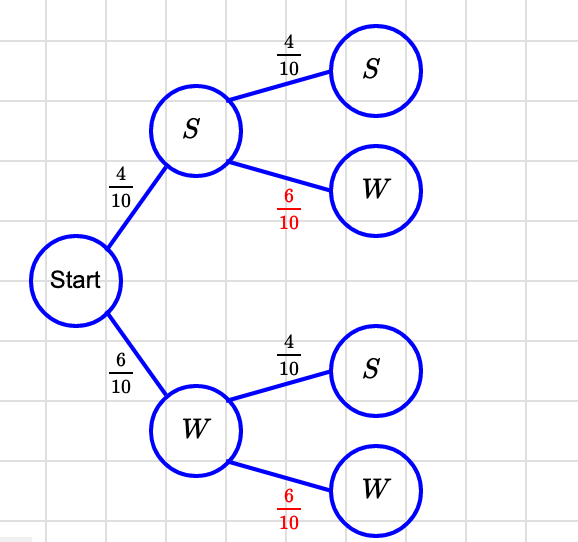
\includegraphics[width=0.35\textwidth]{img/u1}
\end{figure}
Damit sind die bedingten Wahrscheinlichkeiten $P(W|S) = P(W) = \frac{6}{10}$ und $P(S |W) = P(S  ) = \frac{4}{10}$ gleich und somit bei Zurücklegen stochastisch unabhängige Ereignisse.
 \end{frame}


\begin{frame}
    \frametitle{Lösung}
\framesubtitle{}

\begin{figure}[htp]
      \centering
    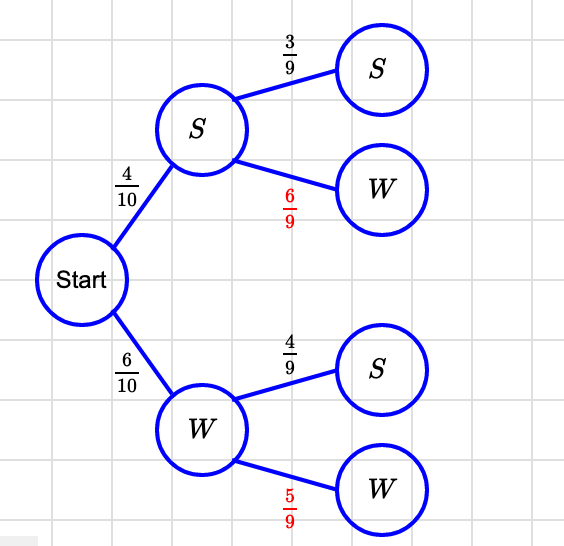
\includegraphics[width=0.35\textwidth]{img/u2}
\end{figure}
Damit sind die bedingten Wahrscheinlichkeiten $ \frac{6}{9} = P(W|S) \neq P(W) =  \frac{5}{9}$  nicht gleich und somit ohne Zurücklegen keine stochastisch unabhängigen Ereignisse.
 \end{frame}

\end{document}
